\documentclass{beamer}
\usetheme{metropolis}
\usepackage{algorithm2e}
\usepackage{amssymb}
\title{Green Resource Allocation Algorithms for Publish/Subscribe Systems}
\subtitle{Distributed Systems Course Paper Presentation}
\author{Artem Tsikiridis}
\institute{cs.grad.aueb}
\date{\today}

\begin{document}

\begin{frame}
\titlepage
\end{frame}

\begin{frame}
\frametitle{Outline}
\tableofcontents	
\end{frame}

\section{Background}
\begin{frame}
\frametitle{Green/Energy Saving Algorithms}

\begin{columns}
\column{0.4\textwidth}
\begin{itemize}
\item Green $\rightarrow$ sustainable energy practices
\item Green IT initiatives are a priority
\end{itemize}

\column{0.6\textwidth}
\begin{figure}
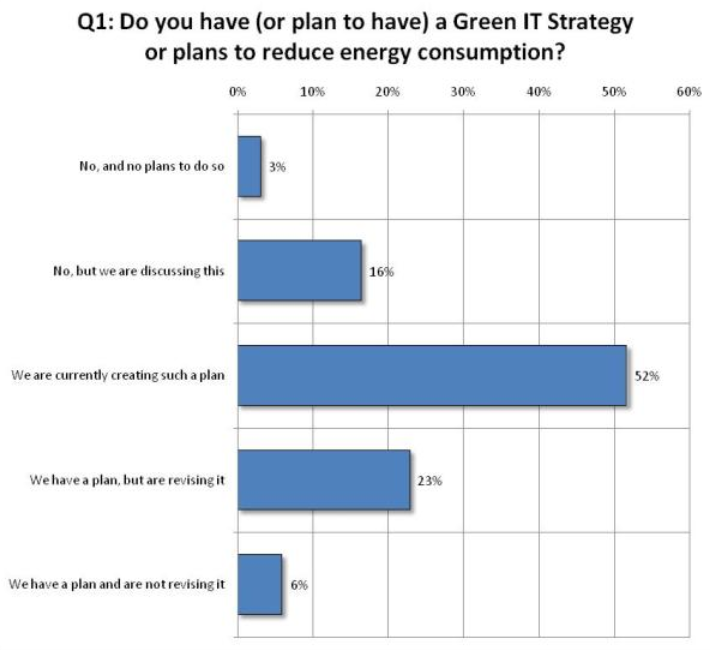
\includegraphics[scale=0.25]{energy_plan_symantec.png}
\caption{source: Symantec Green IT Report, 2009}
\end{figure}

\end{columns}

\textbf{Efficient} use of resources leads to \textbf{lower} IT operational costs.
\end{frame}

\begin{frame}
\frametitle{Message Broker Pattern}
\begin{itemize}
\item Module translating messages from messaging protocol of the sender to messaging protocol of the receiver
\item Widely used in computer networks
\item Minimizes mutual awareness of applications $\rightarrow$ effective decoupling
\item Apache ActiveMQ, Apache Kafka, Celery
\end{itemize}
\begin{columns}
\column{0.5\textwidth}

\includegraphics[scale=0.2]{kafka.png}
\column{0.5\textwidth}

\includegraphics[scale=0.2]{ACTIVEMQ.png}
\end{columns}
\end{frame}

\begin{frame}
\frametitle{Publish/Subscribe Systems}
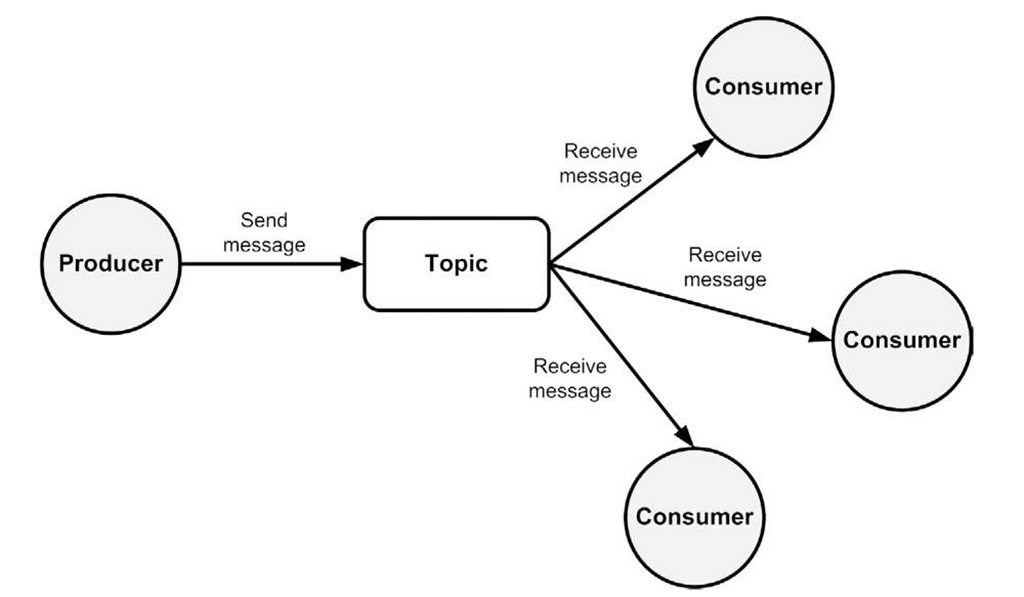
\includegraphics[scale=0.3]{publish_subscribe.jpg}
\begin{itemize}
\item Publishers (senders) put messages to classes
\item Subscribers (receivers) express interest in classes of messages
\item Broker-based systems: publishers post messages to message broker, subscribers register subscriptions with that broker 
\item Used by Green IT implementors, provides network scalability
\end{itemize}
\end{frame}

\begin{frame}
\frametitle{Generic Publish/Subscribe Systems}
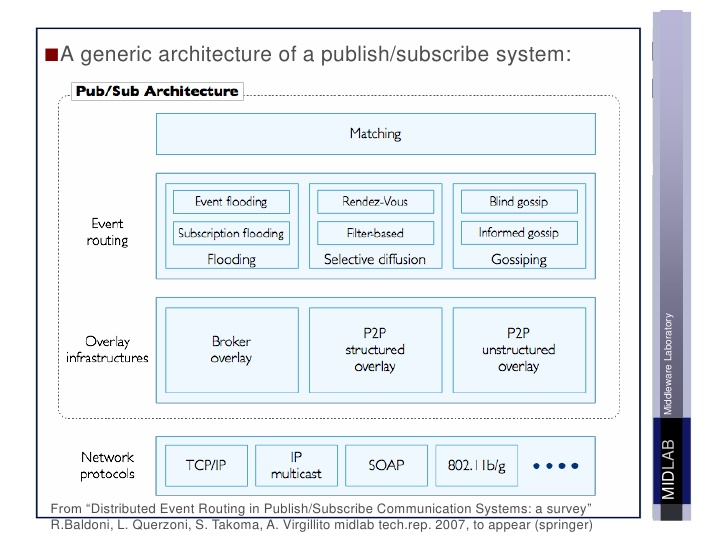
\includegraphics[scale=0.45]{generic_pub_sub.jpg}
\end{frame}



\section{Overview/Prerequisites}
\begin{frame}
\frametitle{Overview}
\underline{Main Goal}: \textbf{minimize} number of brokers, while \textbf{maximizing} resource utilization of allocated brokers 
\begin{itemize}
\item To minimize number of brokers $\rightarrow$ minimize number of messages
\item By minimizing number of brokers $\rightarrow$ minimize size of network
\item As a result, publication hop count is improved (less complexity to place a publication)
\end{itemize}

\underline{How?}
Design and implement a 3-phase scheme to \textbf{reconfigure} the publish/subscribe system.
\end{frame}

\begin{frame}
\frametitle{Phases of 3-phase scheme}
\begin{itemize}
\item\underline{Phase One}: Gathering of performance and workload information from the network using bit-vectors.
\item\underline{Phase Two}: Allocation of subscriptions to brokers using the info from Phase One
\item\underline{Phase Three}: Recursively construct broker overlay with already allocated subscriptions
\item\underline{After 3-phase scheme:} Strategically relocate publishers to new broker overlay
\end{itemize}

Solving an optimization problem which is proven to be $\mathcal{NP}$-complete.

\end{frame}

\begin{frame}
\frametitle{Required components for all phases}
\begin{itemize}
\item \textbf{CROC}: Coordinator for Reconfiguring the Overlay and Clients
\begin{itemize}
\item External pub/sub client
\item Connects to any broker to collect info
\item Executes phases 2 and 3
\item Orchestrates reconfiguration
\end{itemize}
\item \textbf{CBC}: CROC Back-end Component
\begin{itemize}
\item Integrated into each broker
\item Responds to commands sent by CROC (information requests etc.)
\end{itemize}
\end{itemize}
\end{frame}

\section{Phase One}
\begin{frame}
\frametitle{Phase One: Information Gathering}
\begin{itemize}
\item Information gathering protocol implemented using publish/subscribe.
\item CROC connects to first broker $\rightarrow$ sends \textit{Broker Information Request} message
\item Broker broadcasts it to all neighbors
\item Broker replies to CROC with a \textit{Broker Information Answer} when:
\begin{itemize}
\item No neighbors to forward the BIR
\item Has recieved all BIA from other neighbors
\end{itemize}
\end{itemize}
\end{frame}

\begin{frame}
\frametitle{Phase One: BIA}
A Broker Information Answer (BIA) consists of:
\begin{itemize}
\item\textbf{URL}: Useful to reassign subscribers in phases 2 and 3
\item\textbf{Matching delay function}: Linear function enabling CROC to predict input load of broker
\item\textbf{Total Output Bandwidth}: CROC uses it to predict output load of the broker
\item\textbf{Local subscriptions and profiles}: CROC may relocate subscriptions based on that
\item\textbf{Local publishers and profiles}: CROC uses this info to predict load imposed by each subscription
\end{itemize}


Once CROC gets all BIA it executes Phase 2 (reassignment of subscriptions to brokers) and Phase 3(reconfiguration of broker overlay).
\end{frame}

\begin{frame}
\frametitle{Phase One: Subscription and Publisher Profiles}
\textbf{Subscription Profile}: Captures publications sinked by subscription.
\begin{itemize}
\item Allows CROC to accurately estimate load requirements.
\item Generated by broker's CBC
\end{itemize}

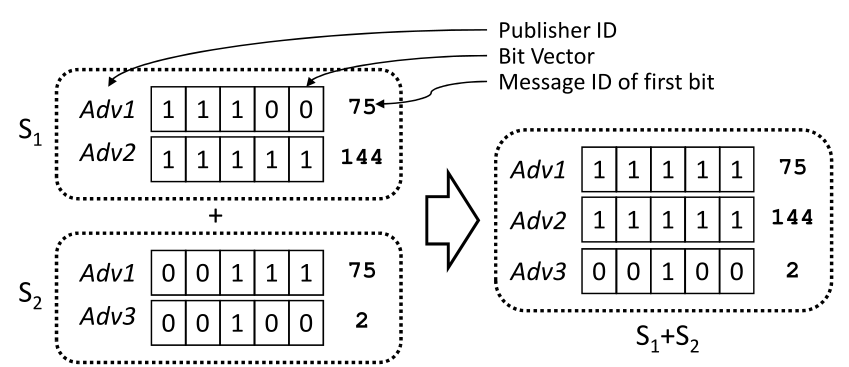
\includegraphics[scale=0.4]{profiles.png}

\end{frame}



\section{Phase Two}
\begin{frame}
\frametitle{Phase Two: Subscription allocation algorithms}
Three proposed algorithms:
\begin{itemize}
\item Fastest Broker First (FSF)
\item Bin Packing
\item Clustering with Resource Awareness and
Minimization (CRAM)
\end{itemize}

\textbf{subscription pool}: All subscriptions reported in BIA in Phase 1.

\textbf{broker pool}: All brokers that sent a BIA message back to CROC

\textbf{Algorithmic Input}: subscription pool, broker pool

\textbf{Algorithmic Output}: set of non-connected brokers (possibly) with allocated subscriptions

\end{frame}

\begin{frame}
\frametitle{Phase Two: Fastest Broker First}
\scalebox{.7}{
\begin{algorithm}[H]
\KwData{subscription pool, broker pool}
\KwResult{set of non-connected brokers (possibly) with subscriptions}

Sort (desc) brokers by total available bandwidth

\While{Subscription pool not empty}{
 s = Randomly pick a subscription
 
 Remove s from pool
 
 Assign s to first broker in list that \textbf{"can handle it"}
 
 \If{s cannot be allocated to any broker}{
 return broker pool
 }
}

return broker pool
\end{algorithm}
}

\begin{itemize}
\item\textbf{broker "can handle" subscription}: Remaining output bandwidth > 0 and incoming publication rate <= max matching rate (BIA Matching delay)

\item\textbf{Complexity}: O(S), S number of subscriptions
\end{itemize}

\end{frame}

\begin{frame}
\frametitle{Phase Two: Bin Packing}
\scalebox{.7}{
\begin{algorithm}[H]
\KwData{subscription pool, broker pool}
\KwResult{set of non-connected brokers (possibly) with subscriptions}

Sort (desc) brokers by total available bandwidth

Sort (desc) subscriptions by bandwidth requirement

\While{Subscription pool not empty}{
 s = Pick first subscription
 
 Remove s from pool
 
 Assign s to first broker in list that \textbf{"can handle it"}
 
 \If{s cannot be allocated to any broker}{
 return broker pool
 }
}

return broker pool
\end{algorithm}
}

\begin{itemize}
\item\textbf{Complexity}: O(Slog(S)), S number of subscriptions
\item FBF and Bin Packing $\rightarrow$ \textit{sorting} algorithms
\end{itemize}

\end{frame}

\begin{frame}
\frametitle{Phase Two: CRAM Metrics}
\begin{itemize}
\item CRAM is significantly different!
\item Relies on the following subscription \textbf{closeness} metrics:
\begin{itemize}
\item \textbf{INTERSECT}: $|S_1 \cap S_2|$
\item \textbf{XOR (inversed)}: $|S_1 \oplus S_2|^{-1}$
\item \textbf{IOS}: $\frac{|S_1 \cap S_2|^2}{|S_1| + |S_2|}$
\item \textbf{IOU}: $\frac{|S_1 \cap S_2|^2}{|S_1 \cup S_2|}$
\end{itemize}

where $S_1$ and $S_2$ are two subscriptions.

\end{itemize} 
\end{frame}

\begin{frame}
\frametitle{Phase Two: CRAM Algorithm}

\scalebox{.7}{
\begin{algorithm}[H]
\KwData{subscription pool, broker pool}
\KwResult{set of non-connected brokers (possibly) with subscriptions}

Run Bin Packing algorithm on Data

\While{True}{
 s1, s2 = Pick two closest subscriptions (using metrics)

 \If{s1 or s2 empty}{
 	return broker pool
 }  
 
 s' = s1 or s2 (bitwise)
 
 Remove s1 and s2 from pool 
 
 Allocate s' using Bin Packing algorithm
 
 \If{Allocation of s' fails}{
 
 	s1, s2 = Revert s1 or s2 (bitwise)
 	
 	Note s1, and s2 should not be clustered again 	
 	
 }
 }

\end{algorithm}
}

\begin{itemize}
\item Complexity: $O(S^3log(S))$
\item Optimizations proposed...
\end{itemize}
\end{frame}

\begin{frame}
\frametitle{Phase Two: CRAM Optimizations}
\begin{enumerate}
\item \textbf{Grouping of Equal Subscriptions}: Consider subscriptions of equal bit vectors identical. Reduce S.
\item \textbf{Search Pruning}: Reduce search space for closeness. $O(S^3log(S)) \rightarrow O(S^2log(S)$
\item \textbf{One-to-Many Clustering}: Cluster $S_1$ with shaded subscriptions before clustering with $S_2$ (even though closeness is worse).
\end{enumerate}

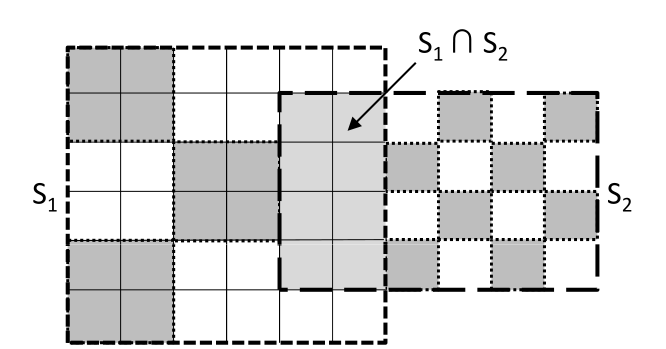
\includegraphics[scale=0.33]{one_to_many.png}

\end{frame}

\section{Phase Three}
\begin{frame}
\frametitle{Phase Three: Recursive Overlay Construction}
\begin{itemize}
\item Design a tree overlay of connected brokers.
\item Use \textbf{CROC} to apply reconfiguration.
\item Finally, use \textbf{GRAPE} algorithm to relocate publishers to the final overlay (out of scope of this paper).
\item Three proposed optimizations for overlay construction.
\end{itemize}
\end{frame}

\begin{frame}
\frametitle{Phase Three: Optimization One}
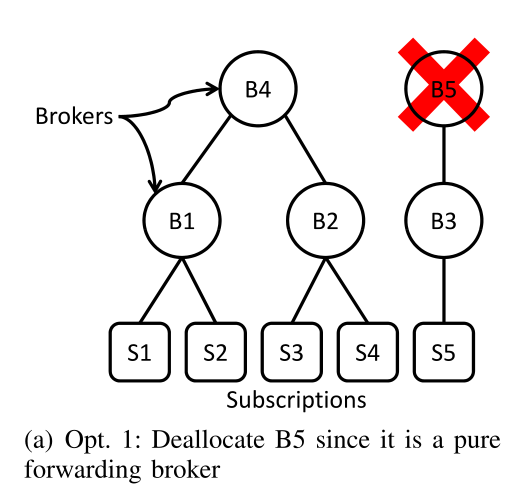
\includegraphics[scale=0.5]{opt_one.png}
\end{frame}

\begin{frame}
\frametitle{Phase Three: Optimization Two}
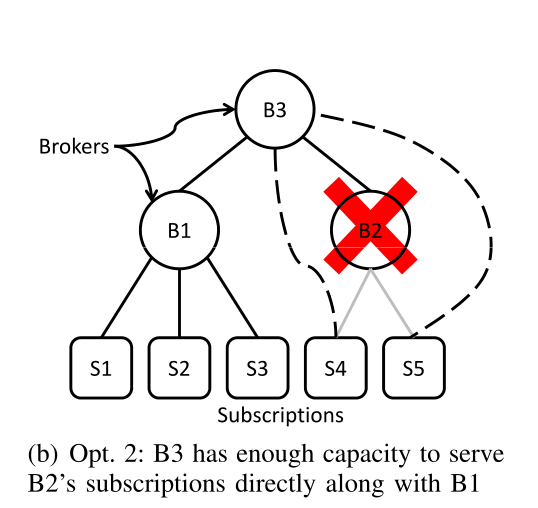
\includegraphics[scale=0.45]{opt_two.png}
\end{frame}

\begin{frame}
\frametitle{Phase Three: Optimization Three}
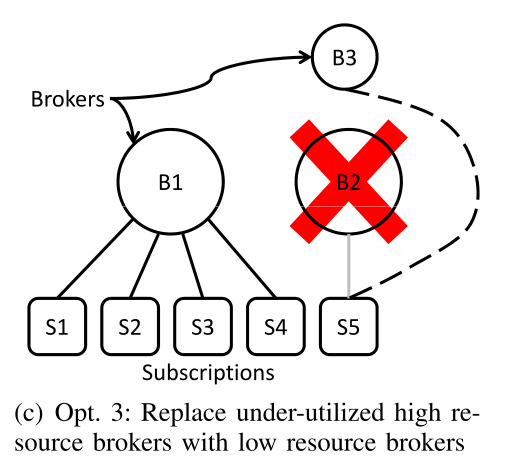
\includegraphics[scale=0.5]{opt_three.png}
\end{frame}

\section{Experiment}
\begin{frame}
\frametitle{Experiment}
\begin{itemize}
\item Comparison of proposed framework with related approaches and baseline algorithms
\item Usage of PADRES, an open-source distributed content-based publish/subscribe system implemented at UToronto

\end{itemize}
\end{frame}

\section{Conclusions}
\begin{frame}
\frametitle{Conclusions}
\begin{itemize}
\item The approach works on any implementation or variation of a pub/sub system.
\item Advantages:
\begin{enumerate}
\item CRAM reduces the average broker message rate by up to 92\% comparing with prior work.
\item CRAM reduces the number of allocated brokers by up to 91\%,
no publication hop.
\item IOU metric heavily reduces computation time of CRAM
\end{enumerate}
\item Disadvantages
\begin{enumerate}
\item CRAM is computationally heavier than all other approaches
\item CRAM may set high delivery delays
\end{enumerate}
\item Possible Remedies
\begin{enumerate}
\item Adjustments to bit vector length (reduce computation time)
\item Strategically relocate publishers to reduce delivery delays
\end{enumerate}


\end{itemize}
\end{frame}

\begin{frame}
Thank you! Questions?
\end{frame}
	
\end{document}
